% RL intro ( introducing helicopter too)
Reinforcement learning is concerned with how agents should take actions in an environment such that the reward is maximized. The policy of an agent (it's behavior) is learned by repeatedly acting in an environment and receiving a reward for each action given the state of the environment. This can be done either by directly improving the current policy, or by directly searching for an optimal policy in the policy space. As interaction with the environment can potentially have high costs, an agent might break down for example, a fundamental issue with this direct policy search is the evaluation of a policy as this often requires multiple trials. A key insight is that many trials are wasted because they do not focus on interesting events to evaluate policies on. 

% TODO: in [ref helictor] for example, such and such results were produced, but in rare event this and that a large room for improvement was present.

% Issue no controllable rare events are tested: solution = co-evolutionary approach
Focusing on controllable rare events (defined in more detail in section \ref{background}) for policy search would improve efficiency significantly. In order to be able to focus on particular events we define an outcome $z$, which specifies the result of every stochastic transition that could occur in a given episode. Thus a given policy $\pi$ and outcome $z$, an episode is deterministic. Instead of wasting random trials on non-informative $z$, this project leverages co-evolutionary principles to evolve both policies $\pi$ aswell as outcomes $z$. The main idea is to improve the evolution process of the population policies by evaluating them on a population of outcomes, which are evolved specially to test the policies.

% Issue evolutionary forgetting
A known issue in co-evolution is co-evolutionary forgetting \cite{forgetting}: policies that excel against new predictors may perform poorly against older ones. This comes from the fact that the new policies only get tested against these new outcomes, but not the older ones. By maintaining a posterior belief, in the form of a gaussian process, over the fitness of policy-outcome pairs previous found results can be remembered. 

\begin{figure}[ht]
  \centering
  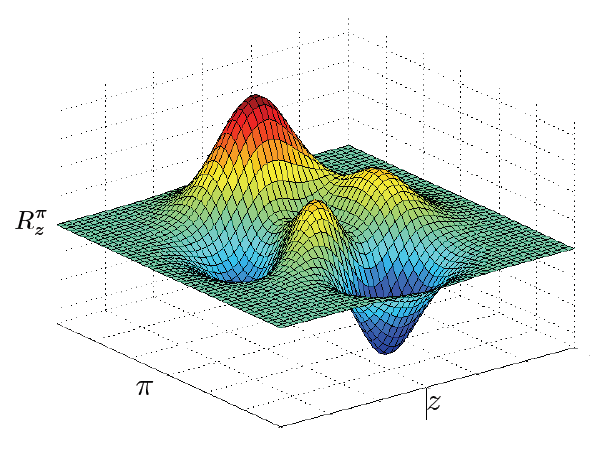
\includegraphics[scale=0.5]{images/fitness-landscape.png}
  \caption{Extended fitness landscape, where the reward is plotted given a policy $\pi$ and outcome $z$}\label{fitnesslandscape}
\end{figure}

% Approach in general
This posterior belief, as shown in figure \ref{fitnesslandscape}, attempts to map policy-outcome pairs to a reward. The challenge in this approach is to select appropriate pairs to evaluate and used to fit, called the acquisition function. Given a appropriate acquisition function, new data points are added to the landscape untill a stop condition is met. Afterwards the best policy is extracted from the gaussian process. \\

% outro: outline rest of paper
In the next section (\ref{background}) the background is provided, followed by related work (section \ref{related}). In section \ref{contrib} our approach is discussed in more detail, after which the experiments (\ref{experiments}) are shown. Lastly the results are discussed (section \ref{discussion}) and concluded (\ref{conclusion}).


